\documentclass[notheorems,mathserif,table,compress]{beamer}  %dvipdfm选项是关键,否则编译统统通不过
%%------------------------常用宏包------------------------
%%注意, beamer 会默认使用下列宏包: amsthm, graphicx, hyperref, color, xcolor, 等等
\usepackage{fontspec,xunicode,xltxtra}  % for XeTeX
\usepackage{verbatim}
\usepackage{mathabx}

%%------------------------ThemeColorFont------------------------
%% Presentation Themes
% \usetheme[<options>]{<name list>}
\usetheme{Madrid}

\useoutertheme{miniframes} 

\usefonttheme{serif}
\setbeamertemplate{background canvas}[vertical shading][bottom=white,top=structure.fg!7] %%背景色, 上25%的蓝, 过渡到下白.
\setbeamertemplate{theorems}[numbered]
\setbeamertemplate{navigation symbols}{}   %% 去掉页面下方默认的导航条.
\usepackage{styles/zhfontcfg}
\usepackage{styles/iplouclistings}
\usepackage{styles/iplouccfg}

%%------------------------MISC------------------------
\graphicspath{{figures/}}         %% 图片路径. 本文的图片都放在这个文件夹里了.
%%------------------------正文------------------------
\begin{document}
\XeTeXlinebreaklocale "zh"         % 表示用中文的断行
\XeTeXlinebreakskip = 0pt plus 1pt % 多一点调整的空间
%%----------------------------------------------------------
%% This is only inserted into the PDF information catalog. Can be left
%% out.
%%%
%% Delete this, if you do not want the table of contents to pop up at
%% the beginning of each subsection:
\AtBeginSection[]{                              % 在每个Section前都会加入的Frame
  \frame<handout:0>{
    \frametitle{Contents}\small
    \tableofcontents[current,currentsubsection]
  }
}

\AtBeginSubsection[]                            % 在每个子段落之前
{
  \frame<handout:0>                             % handout:0 表示只在手稿中出现
  {
    \frametitle{Contents}\small
    \tableofcontents[current,currentsubsection] % 显示在目录中加亮的当前章节
  }
}

%%----------------------------------------------------------
\title{Summary}
\subtitle{Weekly Report}
\author[zhu]{\textcolor{olive}{ZhuYafei}}
\institute[OUC]{\small\textcolor{violet}{Ocean University of China}\\
\small\textcolor{violet}{College of Information Science and Engineering}}
\date{August 22, 2014}
%\titlegraphic{\vspace{-6em}\includegraphics[height=7cm]{ouc}\vspace{-6em}}
\frame{ \titlepage }
%%----------------------------------------------------------


%%----------------------------------------------------------
\section{Scripts}

\begin{frame}
  \frametitle{My first attempt}
  某文件夹下有100个pdf格式的文件,文件按数字1-100命名,如果要在中间加入一个文件27.pdf,那么原文件夹中文件从27开始就要依次加1。
  \begin{itemize}
  \item for $i$ in \$(ls|sort -r); do mv \$$i$\;\;\$[\$\{$i$\%.pdf\}+1].pdf; done
  \item for $((i=100; i>26; i=i-1))$; do mv $\$\{i\}$.pdf\;\;$\$[\$\{i\}+1]$.pdf; done
  \end{itemize}
  \begin{figure}[h]
  \centering
  \centerline{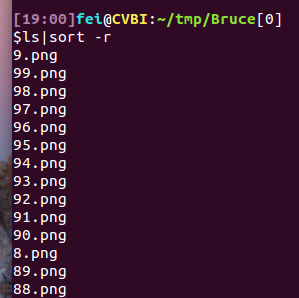
\includegraphics[width=3cm]{sort.png}}
  \end{figure}
\end{frame}


\begin{frame}
  ASD\_GroundTruth文件夹下有1000幅bmp格式的图片,ASD数据集的原图在MSRA\_Stimuli文件夹中,其中有5000幅jpg格式的图片,要从这5000幅图片中找到1000幅与ASD\_GroundTruth文件夹中文件名相同但扩展名不同的图片。
  \begin{itemize}
  \item for $i$ in \$(ls *.bmp); do cp \$\{$i$\%.bmp\}.jpg 文件夹名/; done
  \end{itemize}
\end{frame}


\begin{frame}
  要在某目录下的所有子文件夹中新建相同名字的文件夹。
  \begin{itemize}
  \item for $i$ in \$(ls -l|grep \^{}d|awk `\{print \$9\}'); do mkdir \$\{$i$\}/文件夹名; done
  \end{itemize}
\end{frame}


  两个文件夹下分别有1000幅图片,其图片名不一样,但内容可能一样,编写脚本看其中有多少幅内容是一样的。
\begin{bash}
  #!/bin/bash
  if [ $# != 2 ]; then
	echo -ne "Arguments Error.\n"
	echo -ne "Usage:\n"
	echo -ne "\t$0 <Dir1> <Dir2>\n"
	exit 7
  else
  sum=0
  dir1=$1
  dir2=$2
  for i in $(find ${dir1} -type f)
  do 
	for j in $(find ${dir2} -type f)
	do 
			if cmp -s $i $j
	        	then 
				((sum++))
				echo -ne "${sum}: \033[34m $i \033[0m\t\033[41;33m $j \033[0m\n"
			fi 
	done 
  done
  echo -ne "\n"
  echo -ne "\tThe number of files with same content is \033[41;37m ${sum} \033[0m"
  fi
\end{bash}


  将某文件夹下的所有文件(扩展名都相同)重新按数字命名。
\begin{bash}
  #!/bin/bash
if [ $# != 2 ]; then
	echo -ne "Arguments Error.\n"
	echo -ne "Usage:\n"
	echo -ne "\t$0 <Dir> <Extension>\n"
	exit 7
else
num=1
dir=$1
Extension=$2
for i in $(find ${dir} -type f)
do
	mv $i $dir/${num}.${Extension}
	((num++))
done
fi
\end{bash}


\section{Git使用}


\begin{frame}
  \frametitle{README.md}
  如果所上传的程序直接能运行,一目了然,可以不用写Readme。但如果需要手动添加路径或者程序运行有先后顺序,就要写Readme来让其他使用者更快地了解整个流程。具体格式可下载github上其他人的项目作为参照。当我们从网上下载别人的代码时,也要先看看他们写的Readme,减少自己研究所耗费的时间。
\end{frame}


\begin{frame}
  \frametitle{提交说明}
  正确的版本控制系统的使用方法是,一次提交只干一件事:或是完成了一个新功能,或是修改了一个Bug,或是添加了一幅图片,就执行一次提交。初次提交可以用git commit -m `Initial commit'。
\end{frame}


\begin{frame}
  \frametitle{tmp文件夹}
  当代码出现错误需要进行测试时,可以新建tmp文件夹,在其中放入我们所需要的图片、文件夹等,然后让git忽略这个文件夹,即在.gitignore中加入一行~tmp。为测试这个功能而在工作区所作的修改,可以在测试完成后执行:git checkout -- <file>。
  \begin{figure}[h]
  \centering
  \centerline{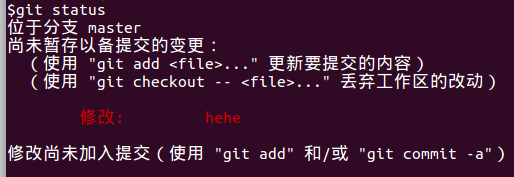
\includegraphics[width=7cm]{44.png}}
  \end{figure}
\end{frame}


\begin{frame}
  当团队中的另一个人在我自己不知道的情况下向远程版本库进行了提交,我没有执行git pull,就修改了本地中的某些文件,并进行push操作,则会出现下面的情况:
  \begin{figure}[h]
  \centering
  \centerline{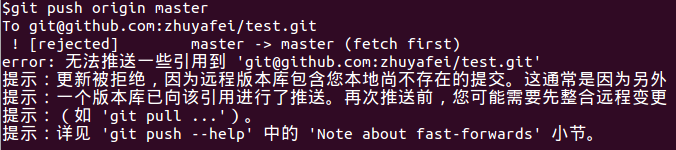
\includegraphics[width=7cm]{11.png}}
  \end{figure}
 执行git pull后出现:
  \begin{figure}[h]
  \centering
  \centerline{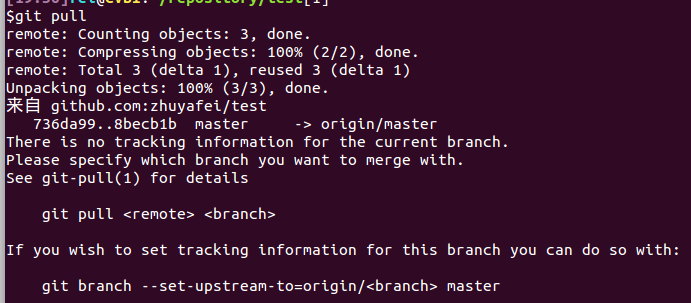
\includegraphics[width=7cm]{22.png}}
  \end{figure}
\end{frame}


\begin{frame}
  执行git pull origin master:
  \begin{figure}[h]
  \centering
  \centerline{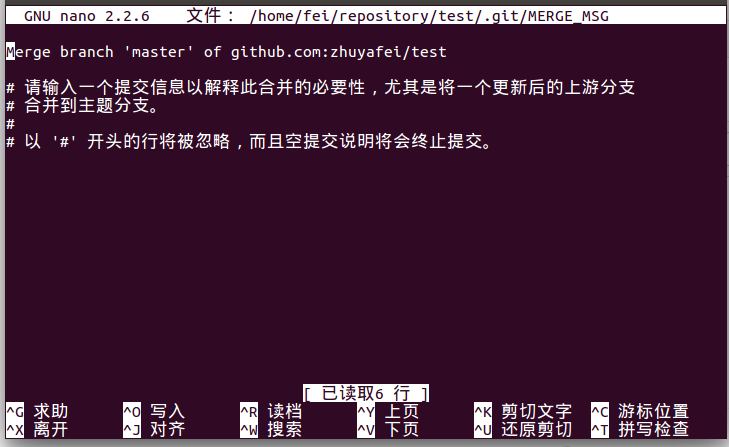
\includegraphics[width=8cm]{33.png}}
  \end{figure}
 最后再重新执行git push origin master。
\end{frame}


\begin{frame}
  \frametitle{问题}
  \,1. git pull = git fetch + git merge, 过程??\\
  \qquad \qquad 2. git暂存区的意义??
\end{frame}


\section{程序书写}

\begin{frame}
  \frametitle{减少运行次数}
  六个算法跑12个数据集得到saliency maps,对每个数据集分别用pr和prf评价:
  $6 \times 12 + 12 \times 2 = 96$\\
  修改后,一个程序跑所有数据集得到saliency maps,再用pr和prf评价:
  $1 + 2 \times 2 = 5$  
\end{frame}


\begin{frame}
  \frametitle{Settings}
  自己写的程序对于不同的输入在程序中要相应地修改某些地方,可以将其设为变量并置于程序开头:

  \%\% Settings\\
  \quad \quad INPUTDATASET=`./Dataset\_Stimuli/';\\
  \quad \quad EXTENSION='*.jpg';\\
  \quad \quad OUTPUTSM=`./Dataset\_SaliencyMaps/'; \\
  \quad \quad \%\% END Settings\\
\end{frame}


\begin{frame}
  \frametitle{小幅度修改他人程序}
  为了看出修改过的地方,一般可以在修改时加上注释。\\
 比如注释掉连续的几行:\\
  \%\% CVBIOUC\\
  \% ***\\
  \% ***\\
  \%\% END CVBIOUC\\
  注释一行:在这行前面加上\%CVBIOUC\%空格
\end{frame}


\begin{frame}
  \frametitle{小幅度修改他人程序}
  添加一段:\\
  \%\% CVBIOUC\\
  echo\\
  \%\% END CVBIOUC\\
  添加一行或修改一行:在这行最后加上空格\%CVBIOUC\% \\
  最好修改之前新建default文件:e.g. cp test.m test.m.default,之后就可以在test.m中操作了。
\end{frame}


\end{document}
